\documentclass[a4paper,11pt]{article}
\pdfoutput=1 % if your are submitting a pdflatex (i.e. if you have
             % images in pdf, png or jpg format)

\usepackage{jheppub} % for details on the use of the package, please
%\usepackage{subfigure}
\usepackage{subcaption}

\usepackage[T1]{fontenc} % if needed
\bibliographystyle{unsrt}

\newcommand{\myunit}[1]{$\, \mathrm{#1}$}

\def\GeV{\ifmmode {\mathrm{\ Ge\kern -0.1em V}}\else \textrm{Ge\kern -0.1em V}\fi}%

\title{\boldmath Design, Construction and Performance Tests of a Prototype Micromegas Chamber with Two Readout Layers in a Common Gas Volume}

\author[a]{Bernard Brickwedde}
\author[a]{Andreas Dulder}
\author[a]{Matthias Schott}
\author[a]{Eda Yildirim}
\affiliation[a]{Johannes Gutenberg-University, Mainz, Germany}

% e-mail addresses: one for each author, in the same order as the authors
\emailAdd{matthias.schott@cern.ch}
\emailAdd{eda.yildirim@cern.ch}

\abstract{
In recent years, micro-pattern gaseous detectors received significant attention in the development of precision and cost-effective tracking detectors in nuclear and high energy physics experiments. The important task for these detectors is not only a precise position measurement, but also the determination of the incoming angle of traversing particles in high rate environments, present for example in the forward region of LHC detectors. One possible realization, using a single Micromegas readout layer, is the so-called Micro-TPC method. However, its angle resolution is very limited, in particular for perpendicular incident beams. A pair of two MicroMegas detectors would allow for a precise angle measurement, however require a relatively large volume.

In this paper, the design and the performance of a prototype detector based on Micromegas technology with two detection layers in a common gas volume will be discussed, suited for small spatial volumes in high rate environments at LHC detectors. Each detection layer has an active area of $9 \times 9$\myunit{cm^2} with a two-dimensional strip readout and is separated by a common gas region with a height of 14 mm. An additional mesh working as an cathode is placed in the middle of the common gas volume separating it into two individual cells. This setup allows for a precise angle reconstruction of incoming particles with a precision of $0.5$\myunit{^\circ} using a detector with reduced material budget, compared to current detector designs. In addition, we present first results of performance studies on the prototype detector based on 4.4\myunit{GeV} electron beam measurements at the test beam facility at DESY. It should be noted that this design reduces multiple scattering which makes the detector also suitable for the measurement of low energy beam experiments.
}

 
\begin{document}

\maketitle
\flushbottom
\newpage

\section{Introduction}
\label{Sec:Intro}
Micromegas detectors are popular in high energy physics experiments due to its ability of detecting charged particles precisely. It is advantageous with its high granularity which allows a precise measurement of the position of a charged particle passing through it and its short signal collection time which allows it to operate at high particle flux experiments such as the LHC. It is also ideal for the large tracking detectors due to its low cost.

The micromegas detectors are under development since it has first built in 1996 \cite{Giomataris:1995fq}. The recent development of micromegas detectors with resistive-strip and two dimensional (2D) readout studied in \cite{Byszewski:2012zz} and \cite{Lin2014281}. In this paper, micromegas detectors are further developed to have two 2D readout layers in a common gas volume (Micromegas Doublet), a prototype is built and its performance is studied. 

This paper starts with introducing the working principle of micromegas detectors (Section \ref{Sec:Principle}) and a typical resistive-strip micromegas with a 2D readout (Section \ref{Sec:MMG}). The layout and the construction of the developed Micromegas Doublet is described in Section \ref{Sec:Detector}. The performance of the prototype is shown in Section \ref{Sec:Performance}. Finally, the conclusion of the study and outlook for possible further measurements/developments are discussed in Section \ref{Sec:Conc}.


\section{Working Principle of Micromegas Detectors}
\label{Sec:Principle}
Micromegas is a parallel plate gaseous detectors which has a drift and amplification gas region separated by a metallic micro-mesh (see Figure \ref{micromegas}). A charged particle passing through the detector ionizes the gas and generates free electrons, due to the electric field in the drift region the electrons drift towards the mesh. The electrons pass through the mesh and enters the amplification region. In order to increase the number of electrons a higher electric field is applied between the mesh and the readout plane (amplification region). In the amplification region the electrons are accelerated enough to create avalanche electrons. Finally, the amplified electrons are collected on the readout strips and processed by a readout electronics.  

\begin{figure}[h!]
	\centering
    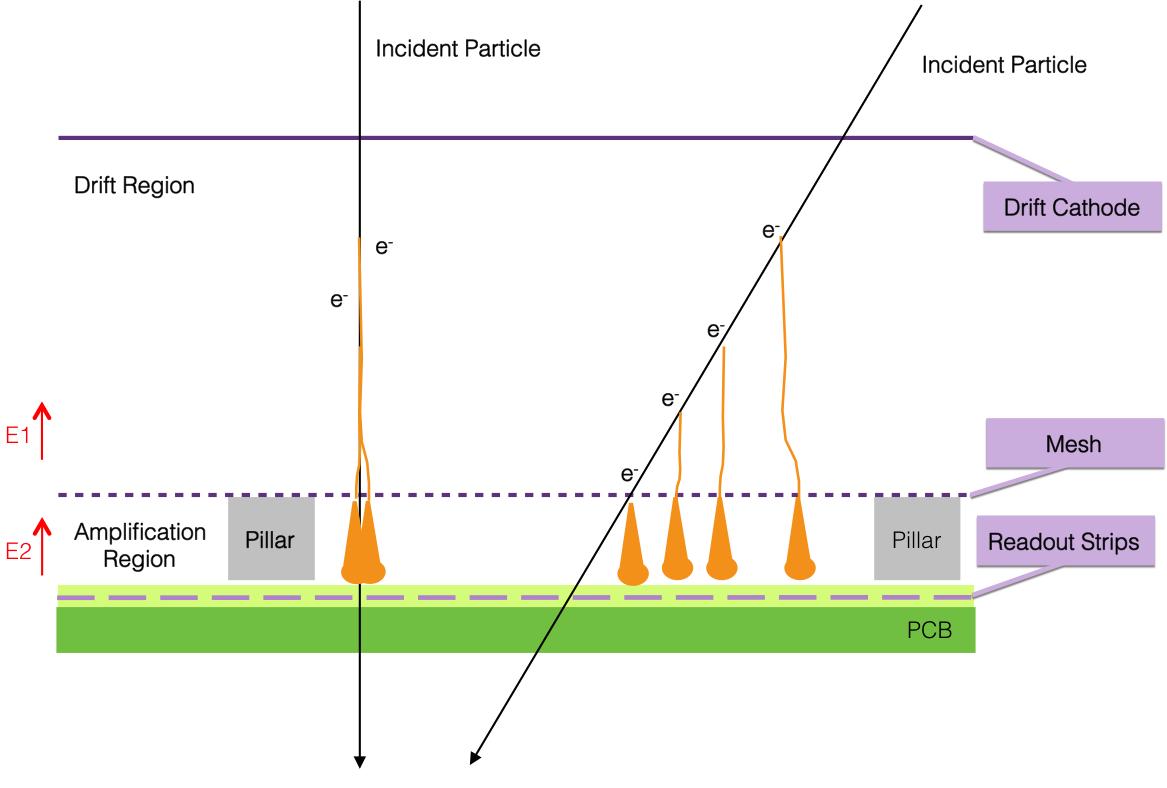
\includegraphics[keepaspectratio=true, width=0.5\textwidth]{Figures/MMG-drawing.png}
	\caption{Working principle of a micromegas detector.}
	\label{micromegas}
\end{figure}




\section{Resistive-Strip Micromegas Detector with 2D Readout}
\label{Sec:MMG}

A typical micromegas detector is few\myunit{mm} thick, with a thin mesh at $\sim 100$\myunit{\mu m} distance to the readout plate. The electric field in the drift region is few hundred\myunit{V/cm} where as in the amplification region it is $\sim 50$\myunit{kV/cm}. In order to achieve high detection efficiency, the amplification factor is kept in the order of $10^{14}$ \cite{Alexopoulos:2011zz}. 

Due to very thin amplification region, micromegas detectors suffers from the possible sparking which may damage the detector and readout electronics. Sparks may also lead to large dead time due to the HV breakdown which would decrease the efficiency of the detector  \cite{Alexopoulos:2011zz}. 

When number of electrons in the avalanche region reaches to Raether limit ($10^{17}$) \cite{Raether1939}. Therefore, any particle (such as low energetic alpha particles) that would create $10^{3}$ electrons in the ionization process would cause a spark in the amplification region. To prevent possible damage caused by sparking, a resistive strip (resistivity few \myunit{M \Omega /cm}) layer and a thin insulator layer on top, is places on the Printed Circuit Board (PCB) as shown in Figure \ref{mmg2D}. The resistive strips causes the avalanche electrons move through them and induces charge on the readout strips \cite{Alexopoulos:2011zz}. The response and the characteristics of this kind of micromegas detector is studied in  \cite{Byszewski:2012zz} and \cite{Lin2014281}.

\begin{figure}[h!]
        \centering
     
         \begin{subfigure}[b]{0.45\textwidth}
   	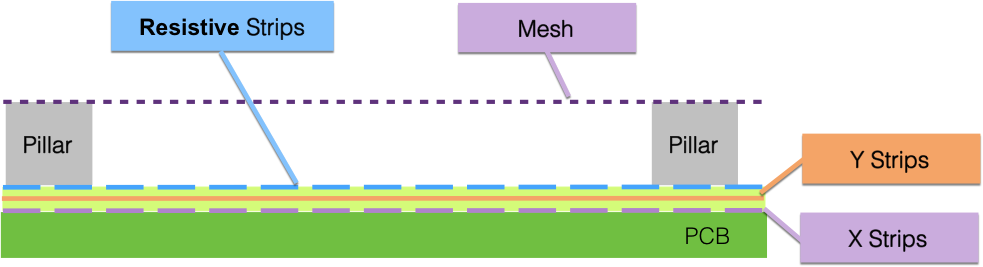
\includegraphics[keepaspectratio=true, width=\textwidth]{Figures/AlongX.png}
	\caption{View along X direction.}
	\label{alongx}
        \end{subfigure}
         ~
         \begin{subfigure}[b]{0.45\textwidth}
        \centering
   	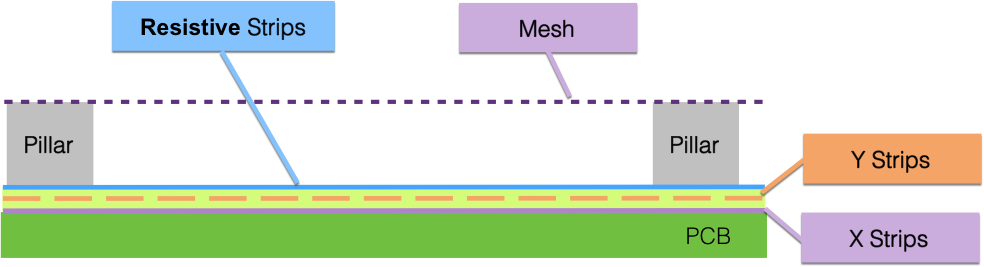
\includegraphics[keepaspectratio=true, width=\textwidth]{Figures/AlongY.png}
	\caption{View along Y direction.}
                \label{alongy}
        \end{subfigure}
         \caption{View of the resistive-strip micromegas detector with 2D readout.}
        \label{mmg2D}
\end{figure}


\section{Detector Layout and Construction}
\label{Sec:Detector}

In this study, a resistive strip micromegas detector with double 2D readout (Doublet) is developed and its characteristics are studied. As shown in Figure \ref{doublet-layout}, the 2D readout planes are placed on top and at the bottom, sharing the same drift region and having their own amplification region. This design reduces the volume that is required for two micromegas detectors. Moreover, it reduces the material budget hence the multiple scattering, which makes the Doublet also suitable for low energy beam experiments. 

\subsection{Detector Layout}
The Doublet has an active region of (WxLxH) $90 \times 90 \times 14$\myunit{mm^3} and is symmetric to the cathode. The electric field in the drift region is $\sim 430$\myunit{V/cm} and in the amplification region is $\sim 43.7$\myunit{kV/cm}. The distance between the cathode and the meshes are $7$\myunit{mm} and between the mesh and readout $128$\myunit{\mu mm}. In the readout plane, X and Y strips are perpendicular and the resistive strips are parallel to the X strips. In both readout planes, there are 360 X and Y strips with a pitch of 250\myunit{\mu m}, the thickness of the X and Y strips are $200$\myunit{\mu mm} and $80$\myunit{\mu mm}, respectively. The resistive strips have the same geometry as the X strips. 


\begin{figure}[h!]
	\centering
    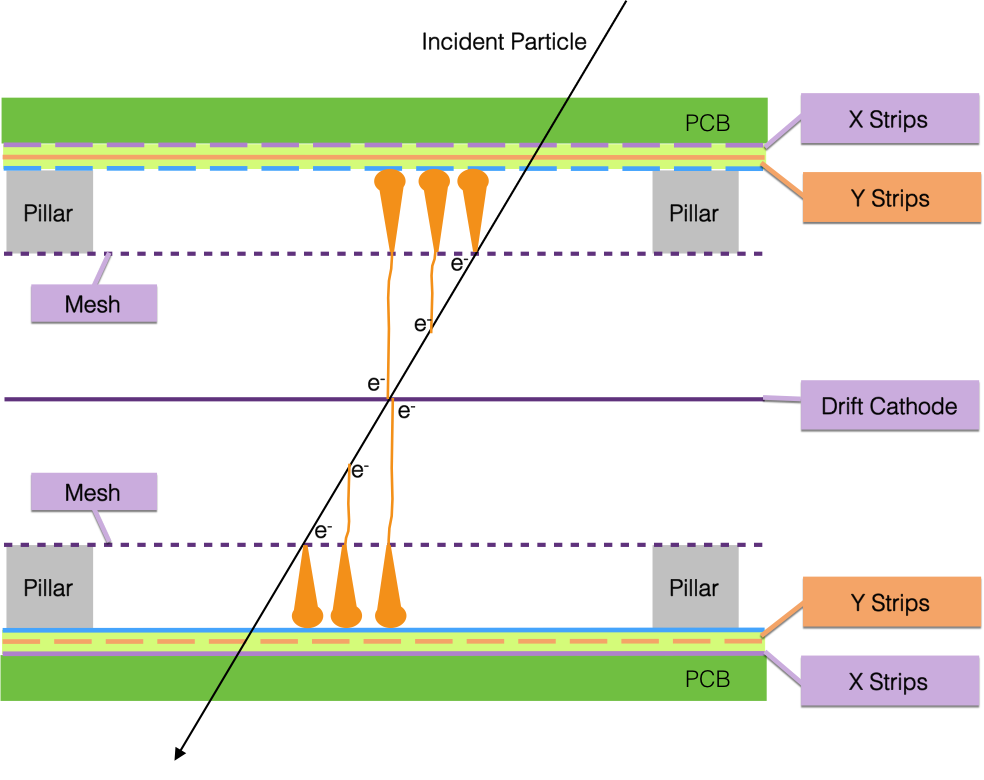
\includegraphics[keepaspectratio=true, width=0.5\textwidth]{Figures/Doublet.png}
	\caption{Detector layout.}
	\label{doublet-layout}
\end{figure}


\subsection{Detector Construction}

The Doublet has assembled as shown in Figure \ref{cons-layout}. There are two aluminum frames each holding a plastic and a brass frame on both sides (shown in Figure \ref{cons-frames}). The meshes are glued on the brass and plastic frames, the cathode mesh is only glued to the upper frames to make the detector possible to re-open. The brass frame is used to set the voltage on the meshes, and plastic frame is used to isolate it from the aluminum frame. Pillars, which have a height of $128$\myunit{\mu m} and a diameter of $350$\myunit{\mu m}, are glued on the readout PCB with a distance of $\sim 2.5$\myunit{mm} to keep a fixed distance between the mesh and the readout PCB to obtain a homogenous electric field in the amplification region. On the edge of the readout layer, an insulator frame is placed to isolate the readout electronics from the voltage on the meshes. In order to make the detector gas-tight, o-rings are placed between the layers.Finally, to prevent the bending of the readout PCB, a sandwich of $0.5$\myunit{mm} FR-4 layers with a $10$\myunit{mm} honeycomb between them is glued on the backside. Finally, all layers are fixed by the help of screws.

\textcolor{red}{\emph{challenges?}}


\begin{figure}[h!]
        \centering
         \begin{subfigure}[b]{0.45\textwidth}
   	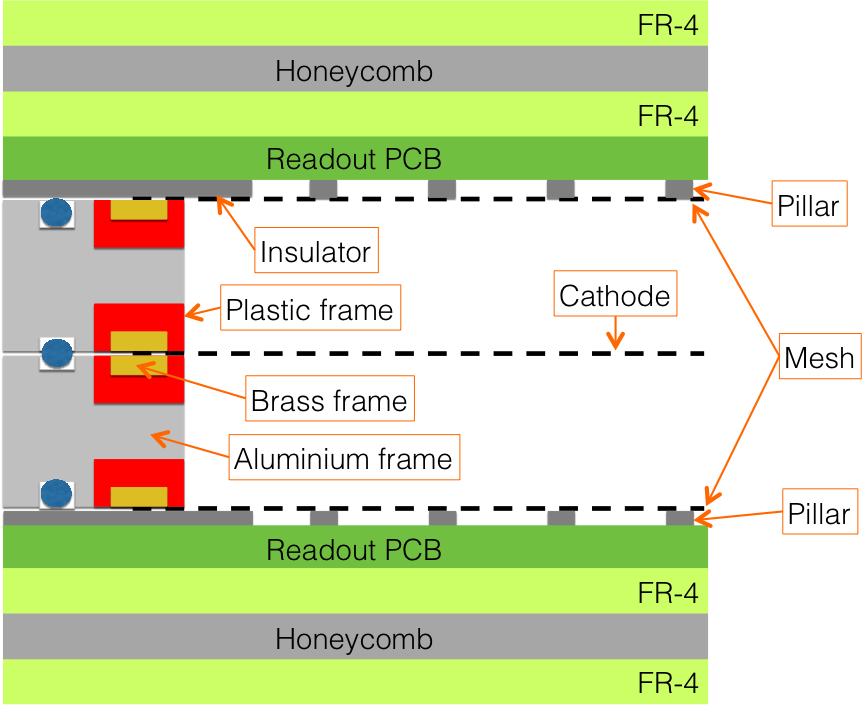
\includegraphics[keepaspectratio=true, width=\textwidth]{Figures/DoubletLayout.png}
	\caption{View from vertical cut (not to scale).}
	\label{cons-layout}
        \end{subfigure}
         ~
         \begin{subfigure}[b]{0.45\textwidth}
        \centering
   	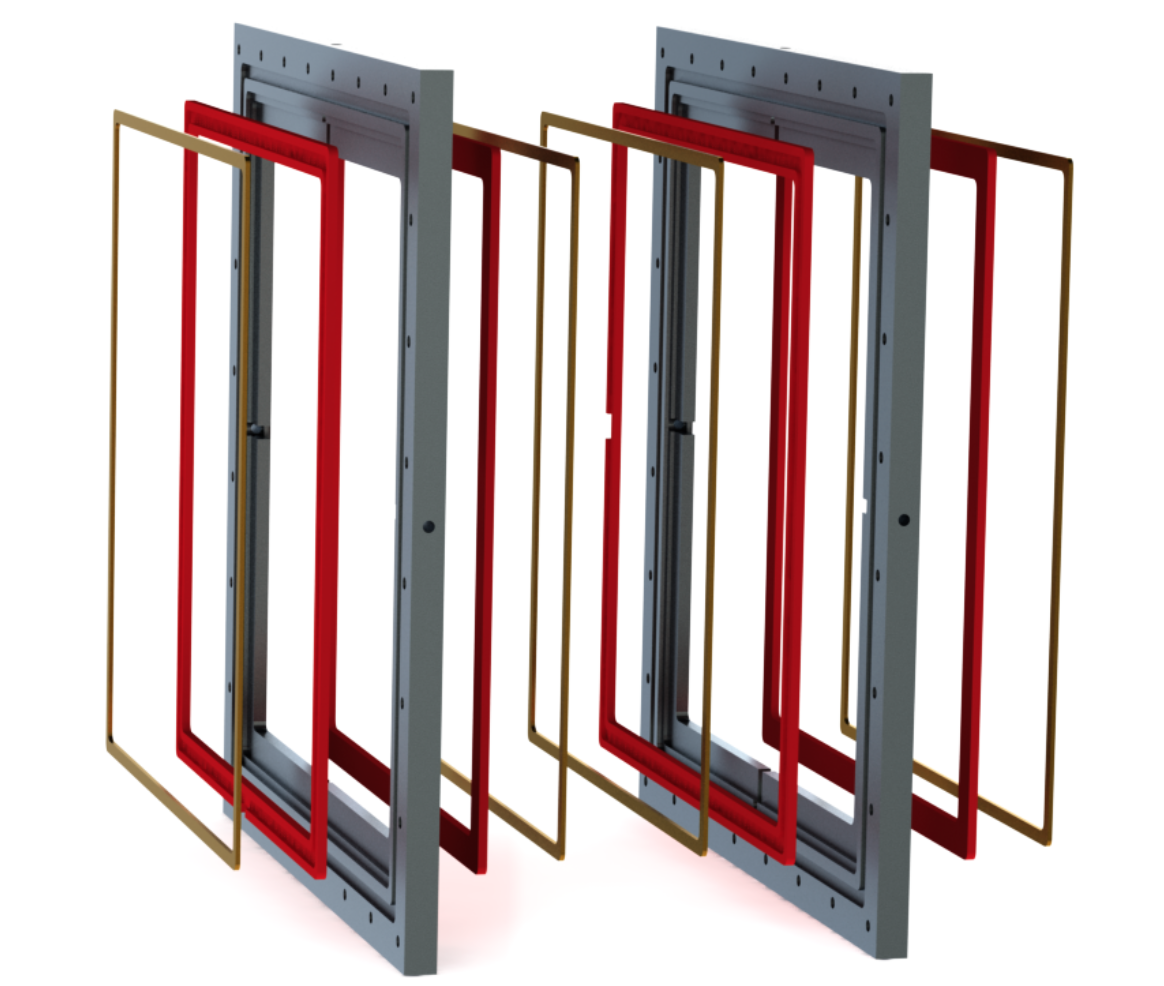
\includegraphics[keepaspectratio=true, width=\textwidth]{Figures/DetFrames.png}
	\caption{View of the frames.}
                \label{cons-frames}
        \end{subfigure}
         \caption{View of the resistive-strip micromegas detector with 2D readout.}
        \label{cons}
\end{figure}







\section{Performance Measurement}
\label{Sec:Performance}
The measurements are taken using 4.4\myunit{GeV} electron beam at DESY II test beam \cite{web-tb}. The Doublet with a reference detector are put under the beam, the setup is shown in Figure \ref{tb-setup}. The reference detector is a typical resistive-strip micromegas detector with 2D readout which was studied in detail in \cite{Lin2014281}. The layout of the setup is shown in Figure \ref{tb-layout}. The Doublet is placed in the upstream and the reference detector in the downstream with a $138$\myunit{mm} distance between them. To study the efficiency, spatial and angular resolution, data taken with different tilt angles around X and Y coordinates. 

\textcolor{red}{\emph{gas mixture}}

\begin{figure}[h!]
        \centering
         \begin{subfigure}[t]{0.45\textwidth}
   	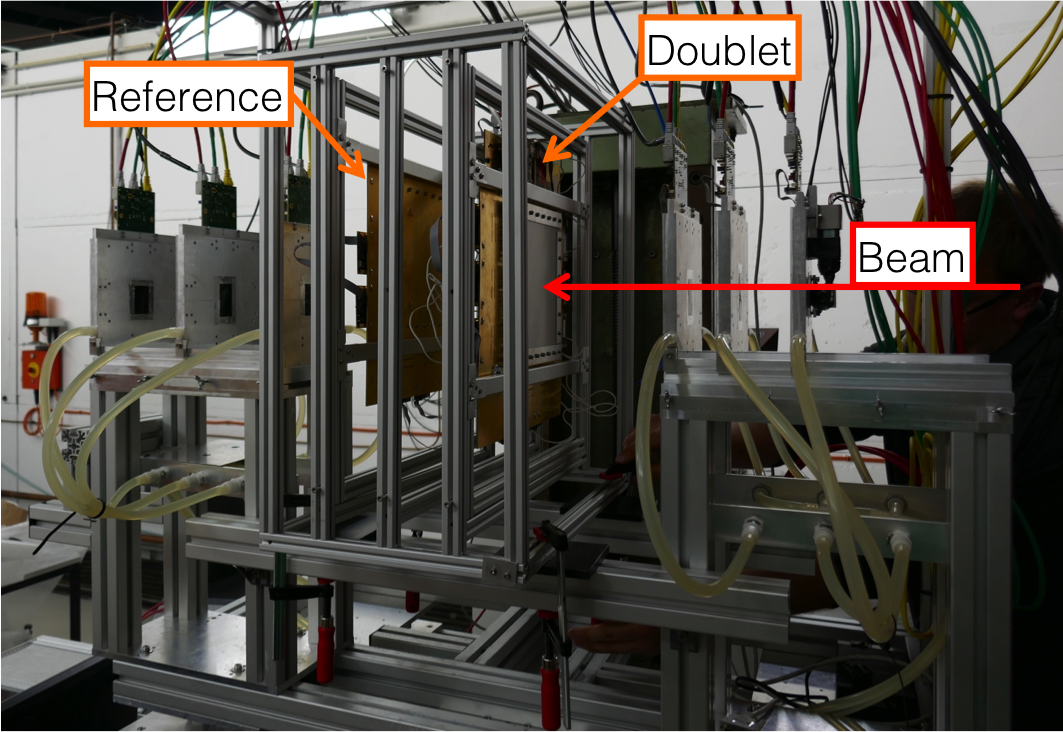
\includegraphics[keepaspectratio=true, width=\textwidth]{Figures/TBsetup.png}
	\caption{Picture of the setup at the test beam.}
	\label{tb-setup}
        \end{subfigure}
         ~
         \begin{subfigure}[t]{0.45\textwidth}
        \centering
   	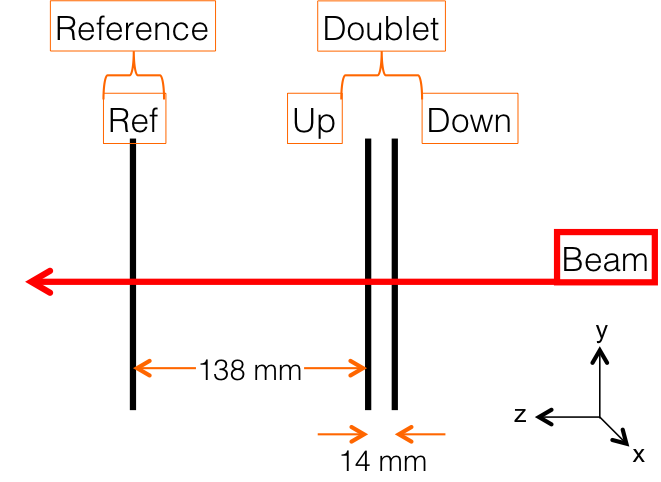
\includegraphics[keepaspectratio=true, width=\textwidth]{Figures/TBlayout.png}
	\caption{Layout of the test beam setup (not to scale).}
                \label{tb-layout}
        \end{subfigure}
         \caption{Setup at the test beam.}
        \label{tb}
\end{figure}

The Scalable Readout System (SRS) \cite{Martoiu:2013aca} that is developed by RD51 Collaboration \cite{web-rd51} is used to readout the both the doublet and the reference detector. It has a discharge protection close to the detector readout electrodes which controls and contains the discharge and prevent it to spread to the rest of the system. It uses the APV25 \cite{APVJones, APVCMS} analog front-end readout chip which was designed for the silicon tracking in CMS. It has 128 input channels that are AC coupled to the detector.  Using HDMI cables, the analog signal from APV25 is transmitted to the back-end board of the SRS DAQ where the signal is process and sent to a PC to be saved for further analysis. 



\subsection{Signal Characteristics}

The APV25 chips measures the signal in a channel 27 times with a time step of 25\myunit{ns}. The height of the signal (in ADC) is proportional to the collected charge on the readout channel at the corresponding time. The signal evaluation in time on X and Y strips in an event is shown in Figure \ref{sigvstime}. As mentioned before, the avalanche electrons propagate over the resistive strips and induces charge on the X and Y readout strips. Since Y strips are perpendicular to the resistive strips, the charge propagate along Y strips and induces charge on more strips compared to the induction in X direction. The total measured signal on X strips are smaller than the ones on Y strips due to the distance between X and resistive strips.


\begin{figure}[h!]
        \centering
         \begin{subfigure}[b]{0.45\textwidth}
   	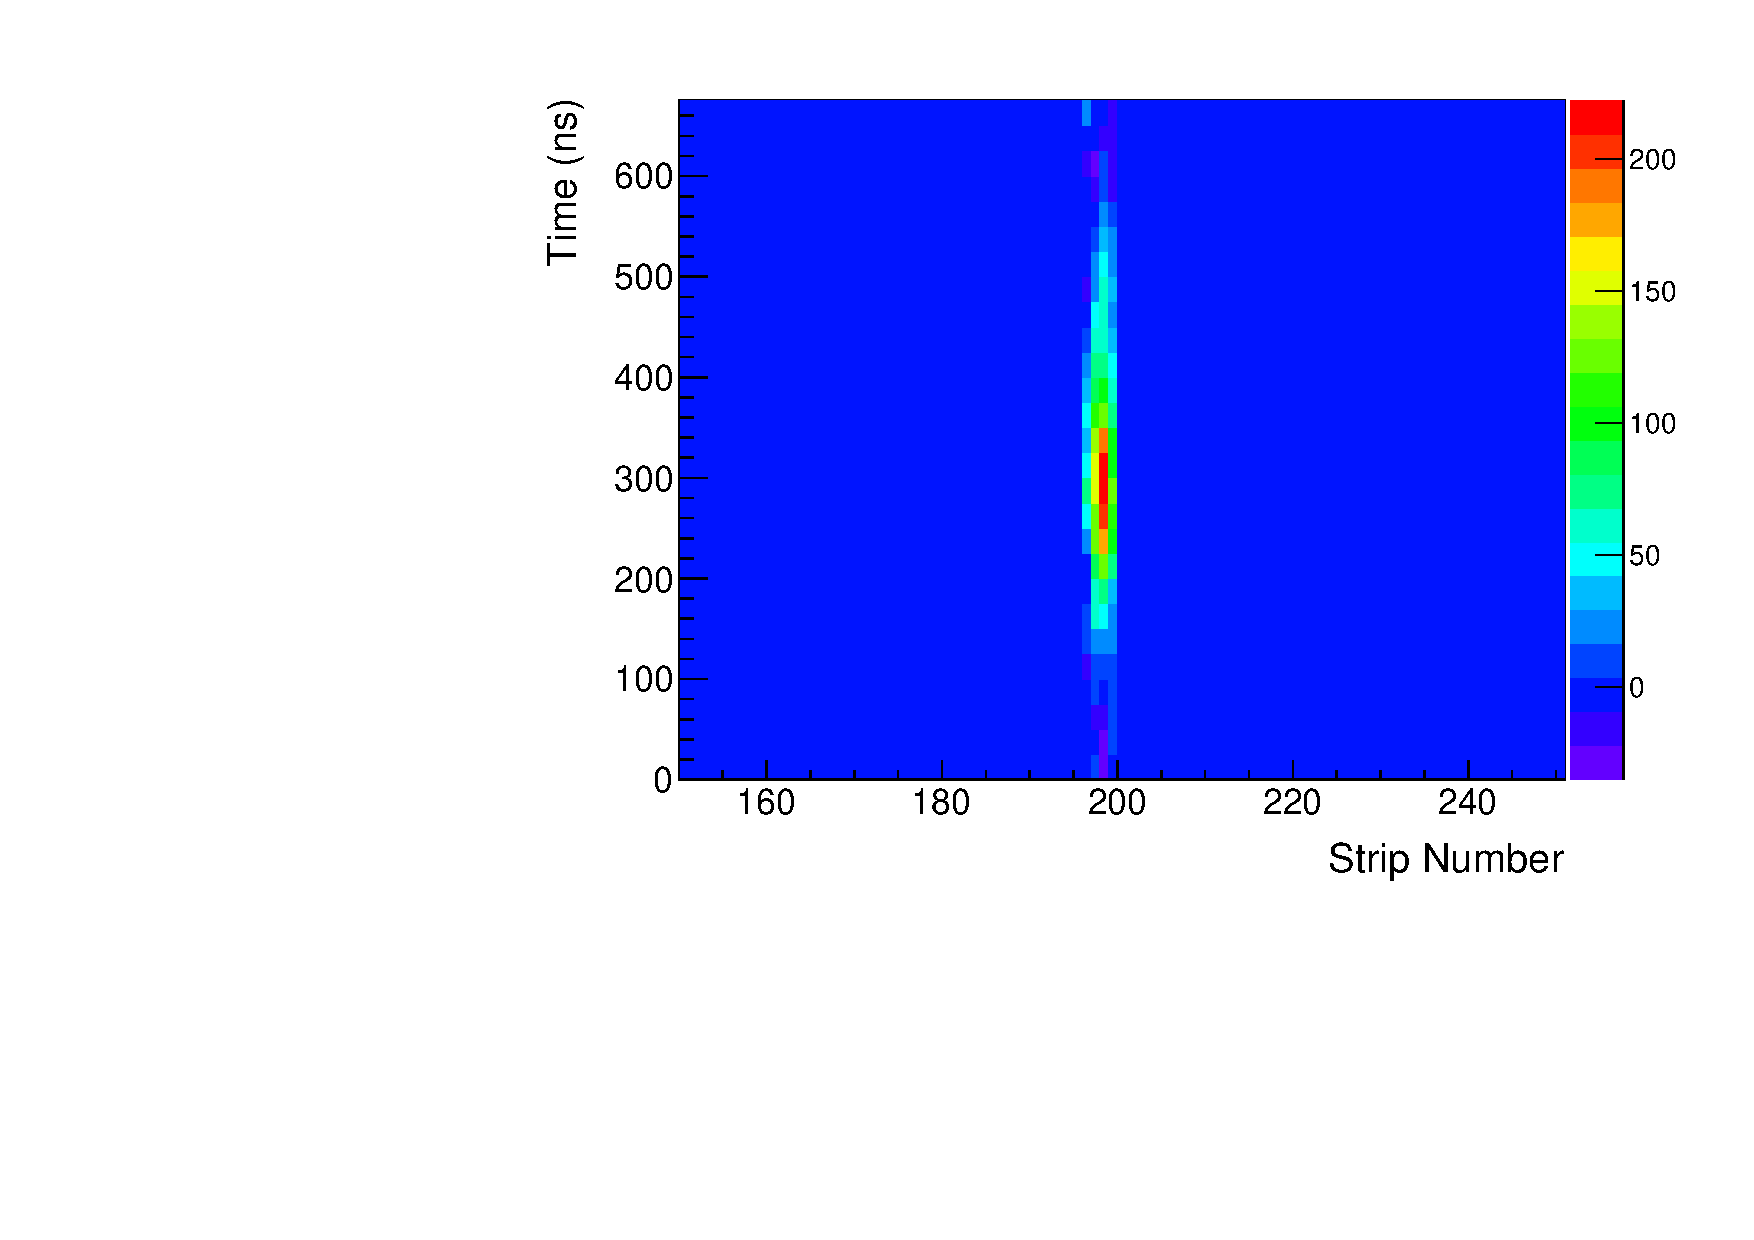
\includegraphics[keepaspectratio=true, width=\textwidth]{Figures/event_13DownX_timeVSchannel.pdf}
	\caption{On X strips.}
	\label{sigvstime-X}
        \end{subfigure}
         ~
         \begin{subfigure}[b]{0.45\textwidth}
        \centering
   	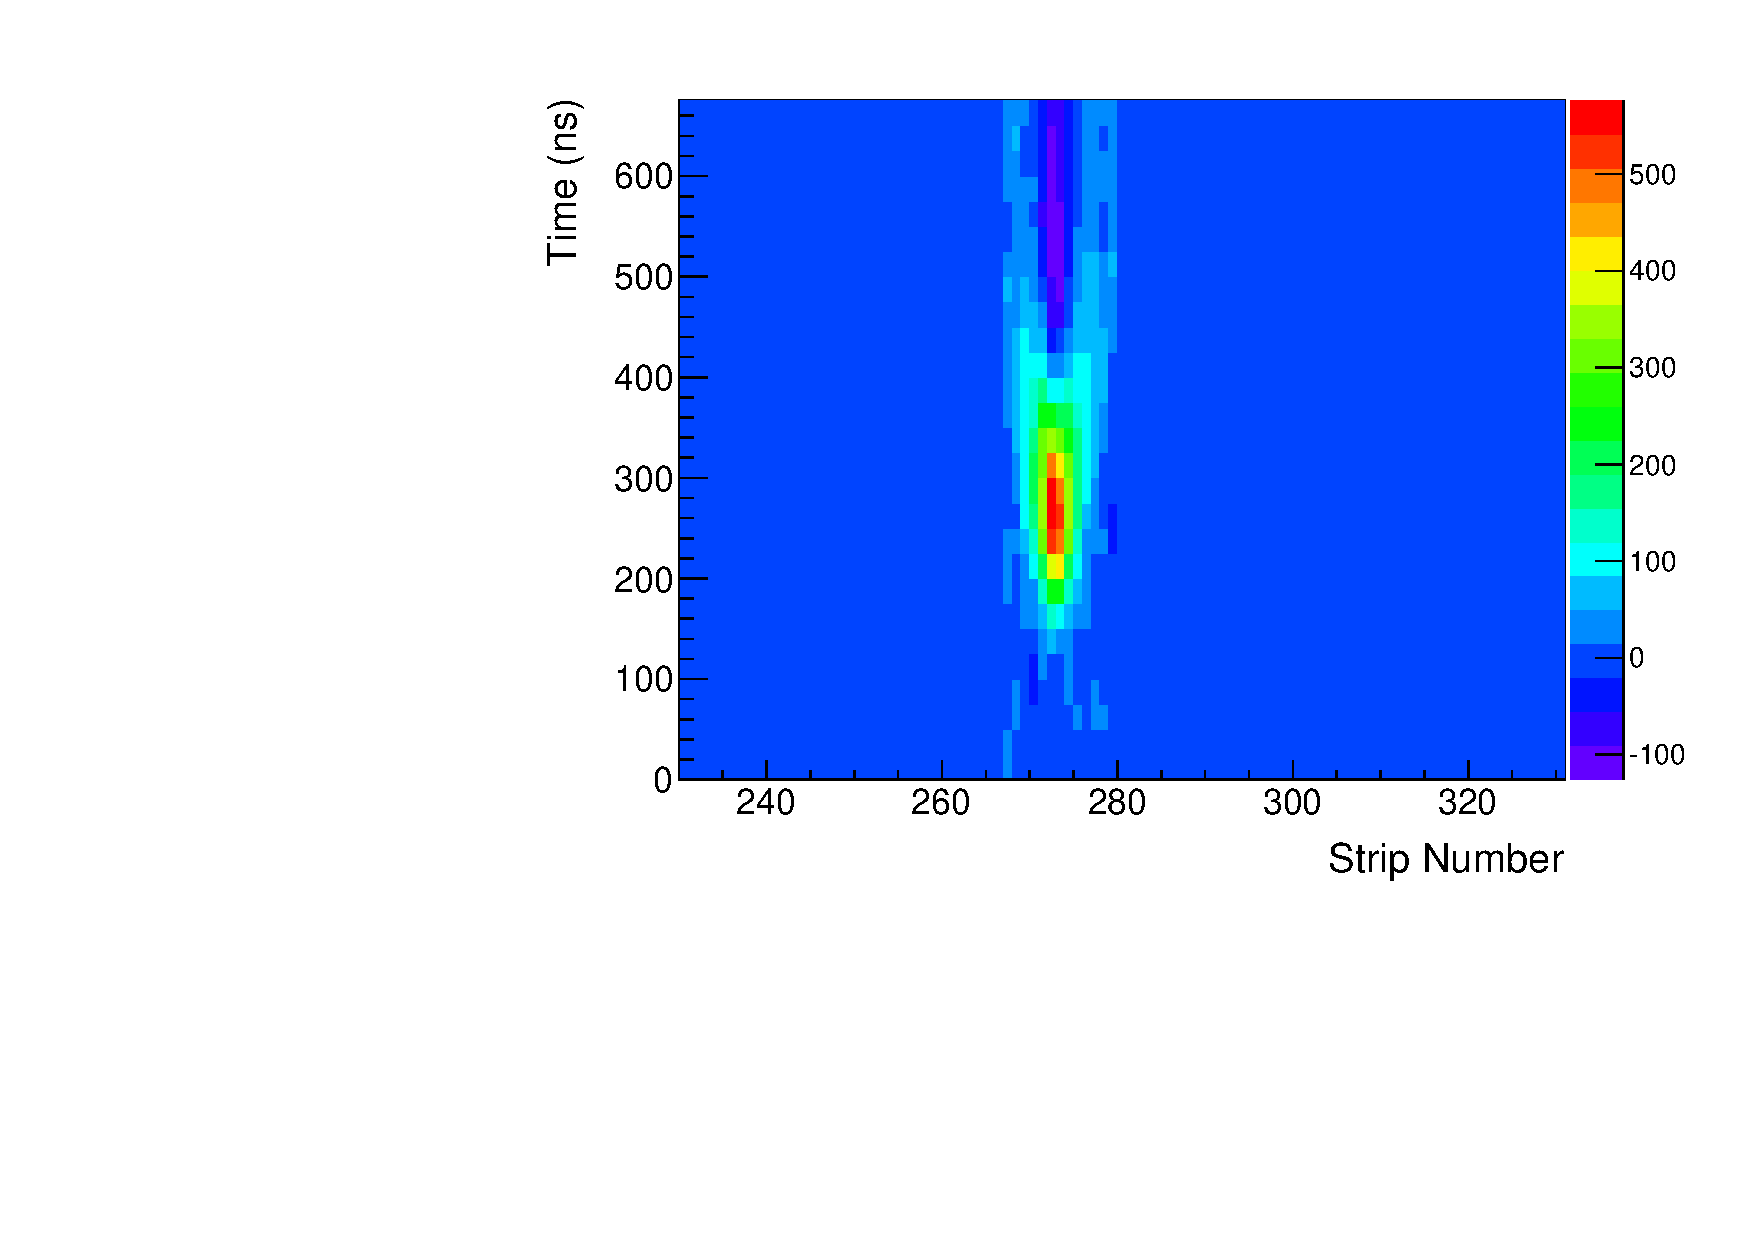
\includegraphics[keepaspectratio=true, width=\textwidth]{Figures/event_13DownY_timeVSchannel.pdf}
	\caption{On Y strips.}
                \label{sigvstime-Yt}
        \end{subfigure}
         \caption{Signal distribution over time.}
        \label{sigvstime}
\end{figure}

Strips that have less than 20\myunit{ADC} are considered as noise and the rest have clustered to calculate the hit position. Clusters have required to include more than 2 strips. Alignment of the planes are performed using a data run that is perpendicular to the beam direction and applied to all data runs. As can be seen in Figure \ref{cons-layout}, the Y coordinate of Up layer is parallel to the X coordinate of Down layer. Therefore, the analysis is performed after transforming local coordinates to the global coordinates defined by reference detector.

\subsection{Efficiency Measurements}

In order to calculate the efficiency of a layer, tracks are defined using the hits on the other two layers and searched for a hit on the layer that the efficiency calculated for. Figure \ref{eff} shows the efficiency of each layer if the Doublet as well as the Reference detector. The calculated efficiencies of the Reference detector are higher than $95\%$ which is consistent with the measurement performed before \cite{Lin2014281} with this detector. The layers that are closer to the amplification region (RefY, UpX, DownY) has slightly higher efficiency than the layers that are far from amplification region. This is due to the resistive strips as well as the material between the layers which reduces the induction on the local X strips. The efficiencies calculated with different tilt angles are similar for over the different data runs taken with various tilt angle. For DownX layer, while there is no significant dependence on the tilt angle around X coordinate, some dependence has observed for tilt around Y coordinate. The reason might be the bending of the amplification mesh used for Down layer. When the detector opened, it has seen that the mesh has bended forming a wave structure in one direction.

%In this study, the layers that are close to the resistive strips are measured, these layers are DownX and UpY in global coordinates. Figure \ref{eff} shows that these layers have $\sim 99\%$ efficiency independent of tilt of the detector.

\begin{figure}[h!]
        \centering
         \begin{subfigure}[b]{0.45\textwidth}
   	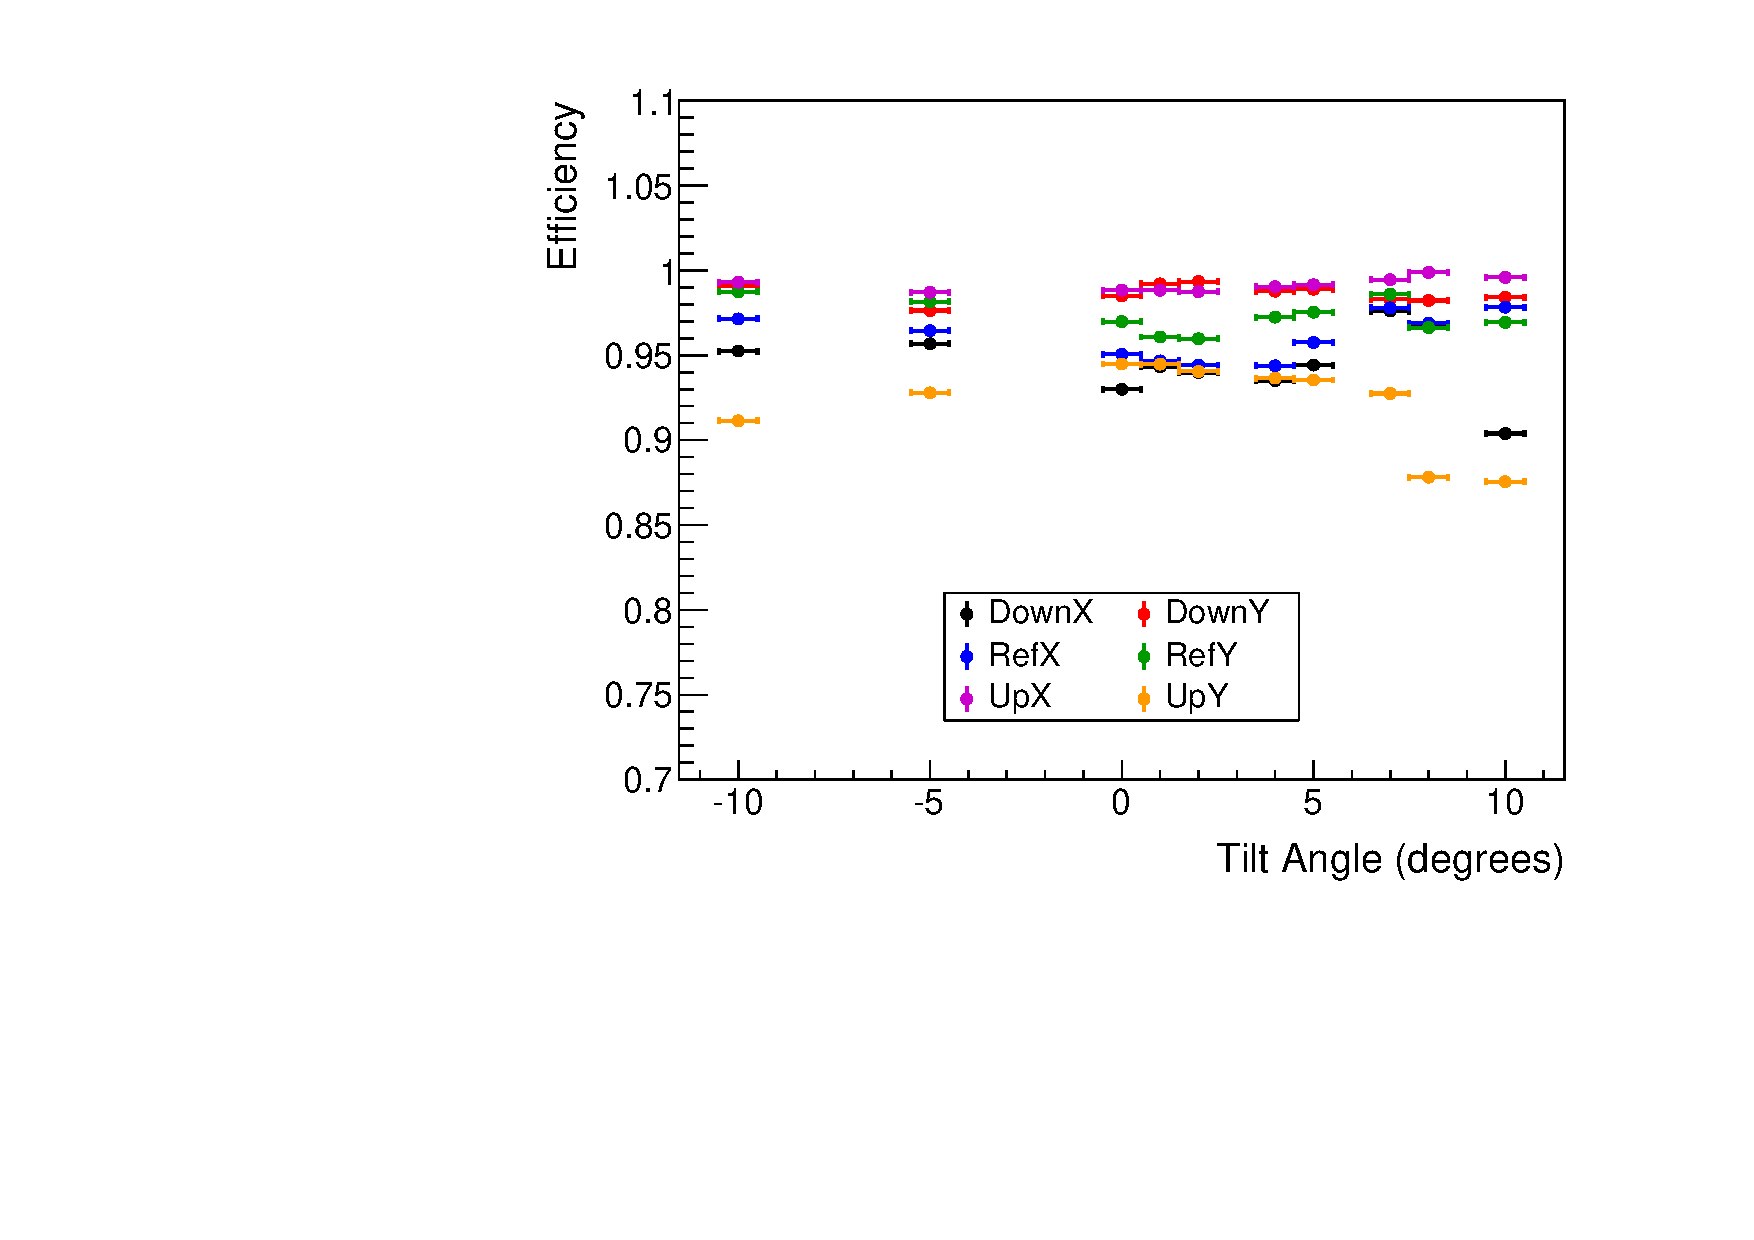
\includegraphics[keepaspectratio=true, width=\textwidth]{Figures/mgr_eff_tiltX.pdf}
	\caption{Tilt around X coordinate.}
	\label{eff-X}
        \end{subfigure}
         ~
         \begin{subfigure}[b]{0.45\textwidth}
        \centering
   	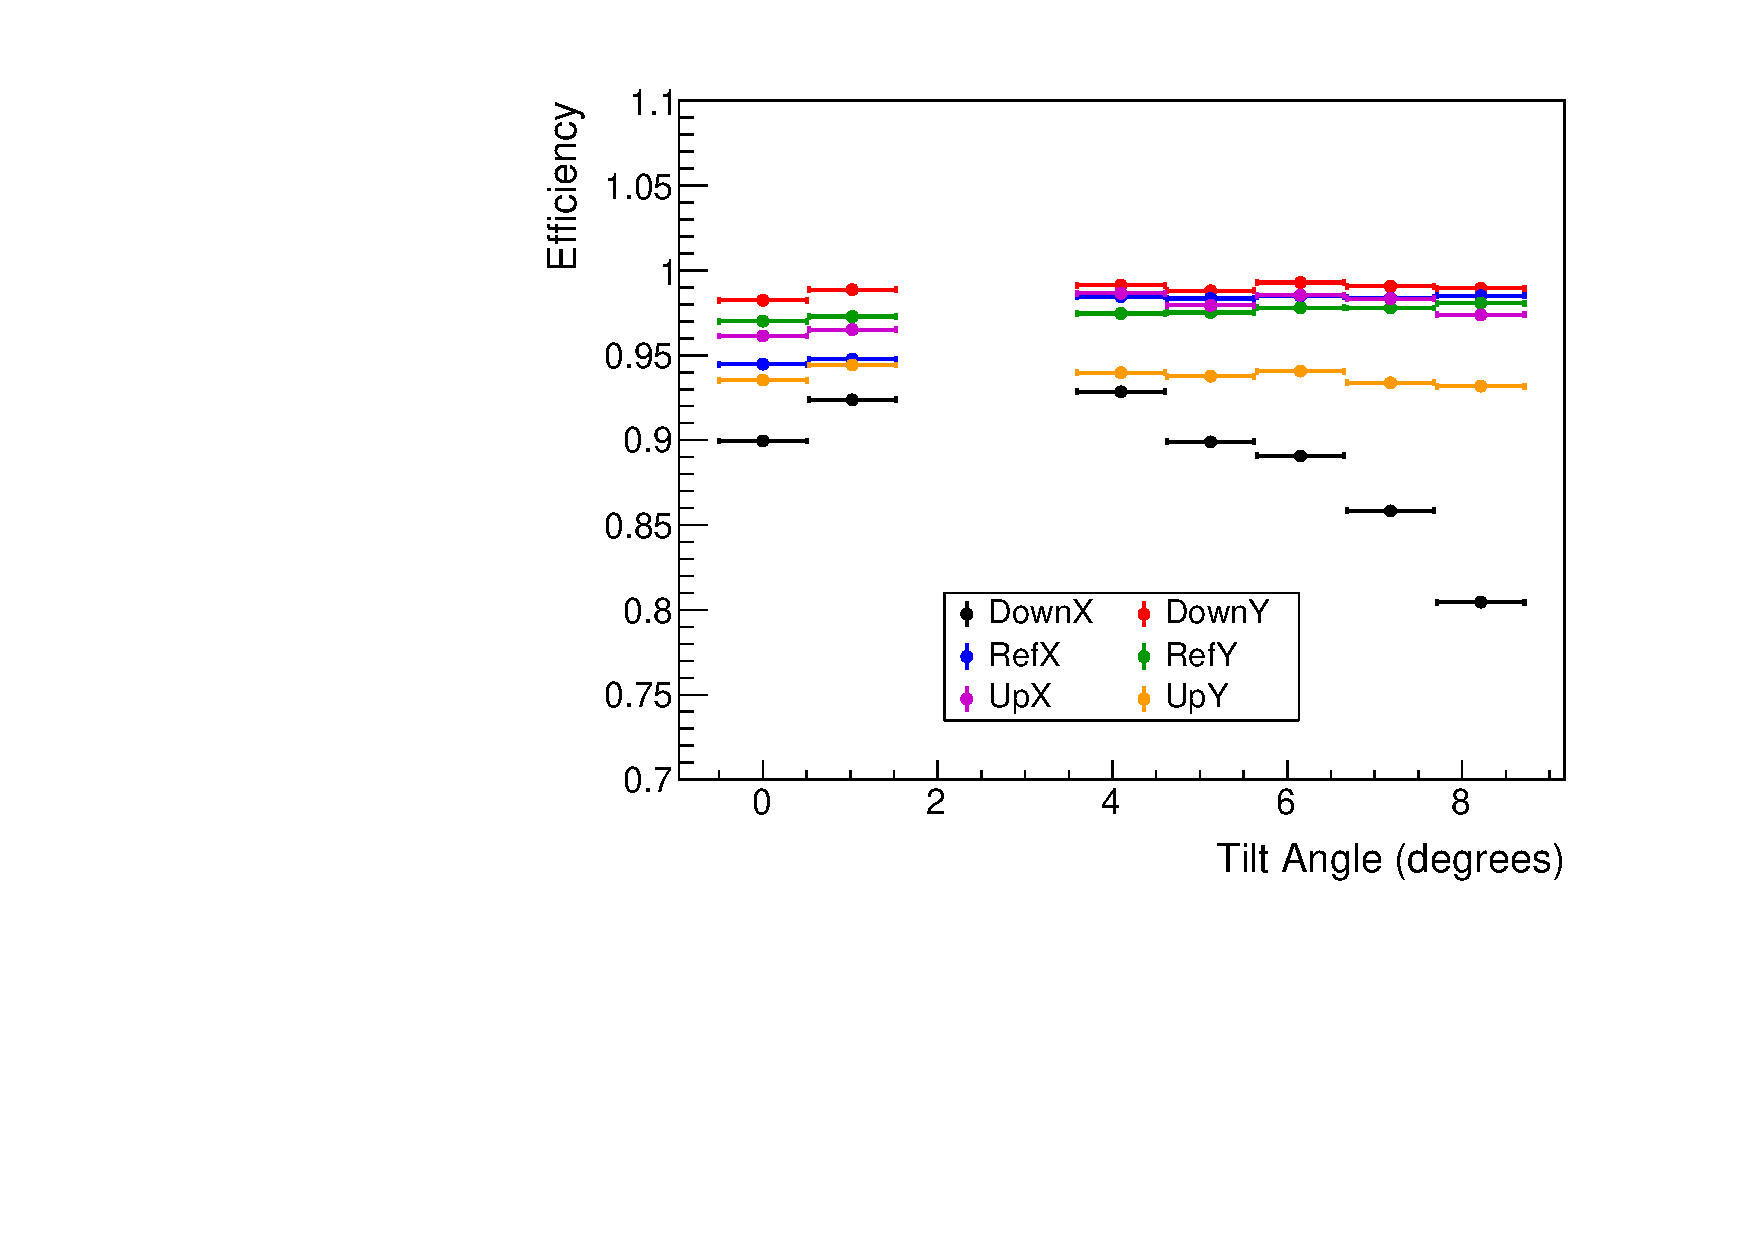
\includegraphics[keepaspectratio=true, width=\textwidth]{Figures/mgr_eff_tiltY.pdf}
	\caption{Tilt around Y coordinate.}
                \label{eff-Y}
        \end{subfigure}
         \caption{Hit efficiency dependence on tilt angle.}
        \label{eff}
\end{figure}

\subsection{Spatial Resolution}
\label{sec-spa-res}
Spatial resolution is calculated by defining tracks using hits on two layers, by extrapolating the track to the third layers position expected hit position is determined by the intersection point. Figure \ref{dx} shows the residual distribution of the Down layer of the Doublet in X and Y coordinates when the detector was tilted by 4 degrees around Y axis. The residuals (dx, dy) are the difference of expected and measured hit positions. The spatial resolutions are obtained from the deviation of the residual distribution. The offset on the residuals due to the mis-alignment which do not effect the resolution measurement. The systematic error is calculated by performing two fits to the distribution, the red line shows the gaussian fit where the blue one is for the gaussian+a constant. The difference in the deviation obtained by these two fits are taken as a systematic error.

\begin{figure}[h!]
        \centering
         \begin{subfigure}[b]{0.45\textwidth}
   	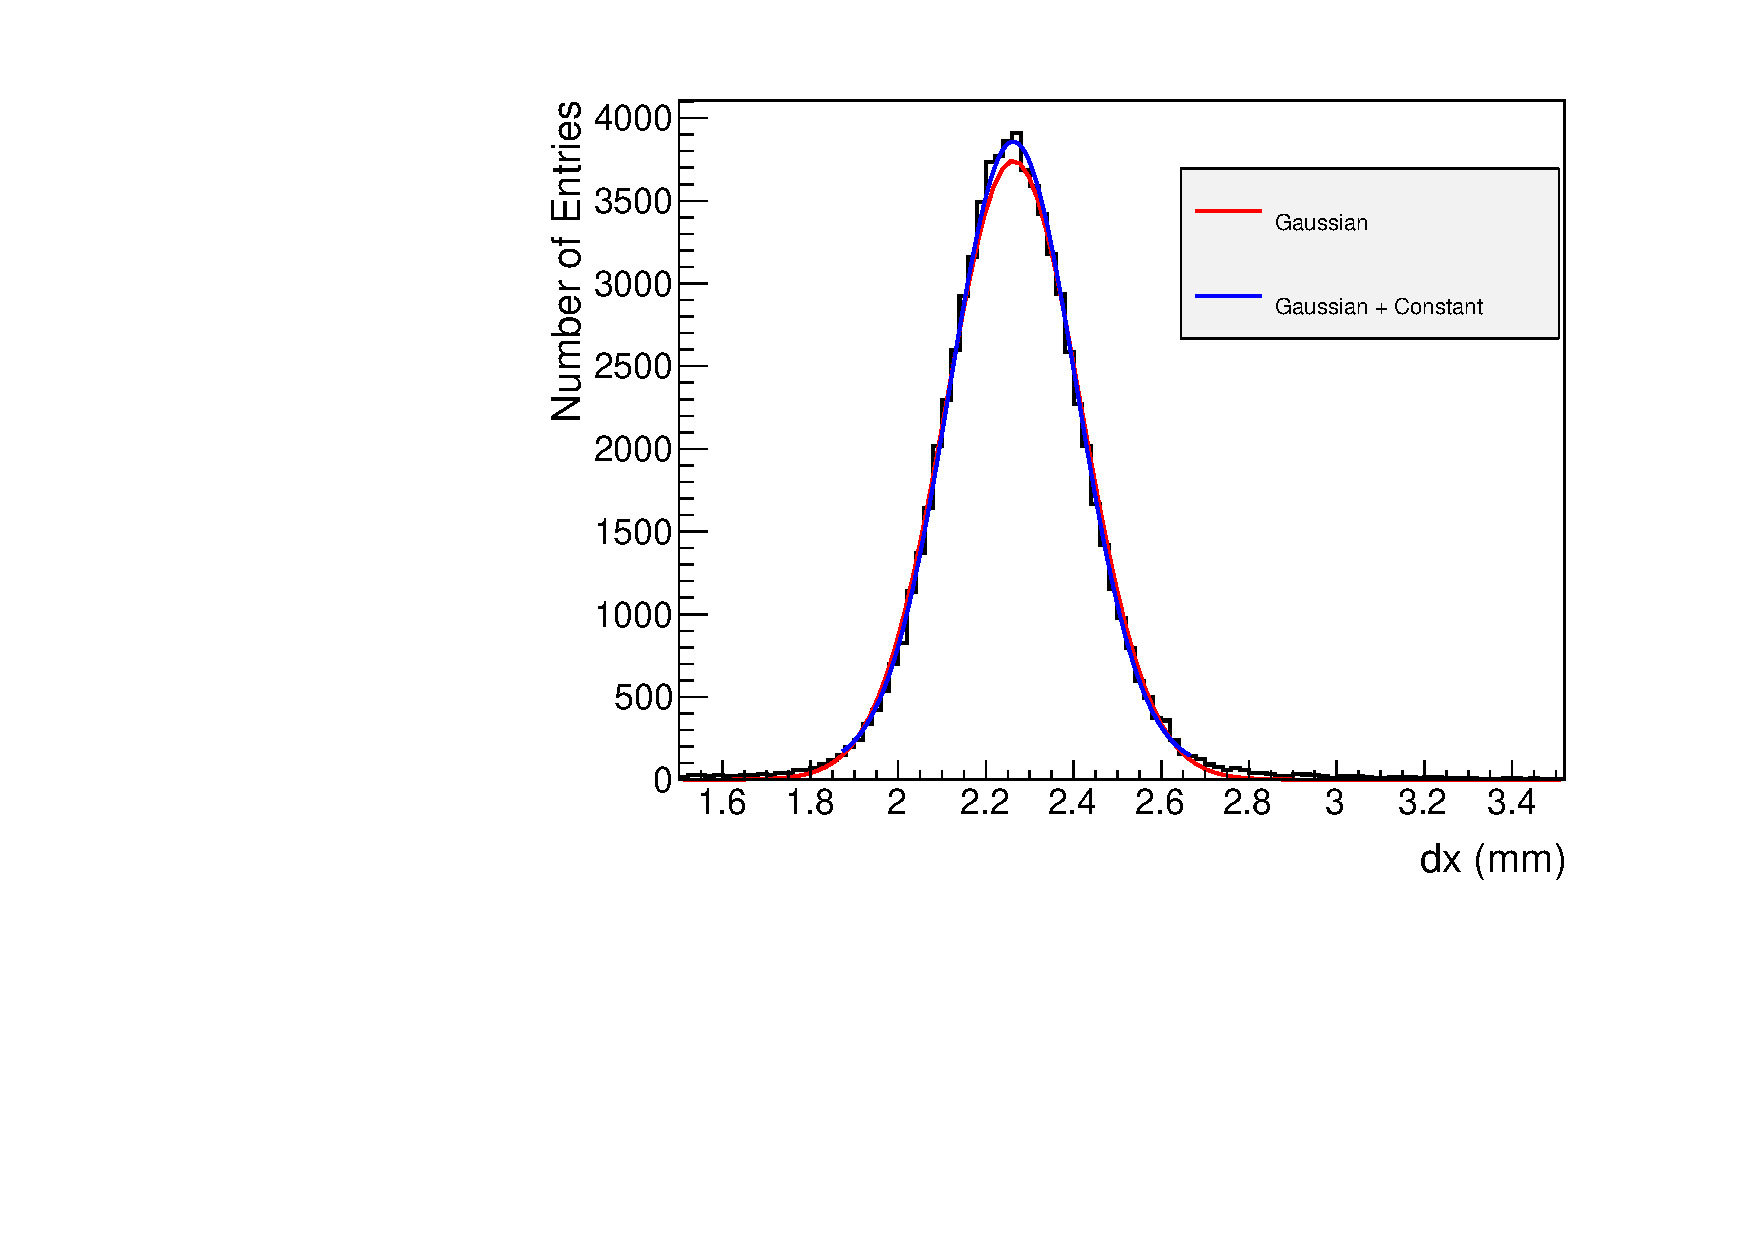
\includegraphics[keepaspectratio=true, width=\textwidth]{Figures/spatialRes_DownX.pdf}
	\caption{Spatial residual of DownX.}
	\label{dx-X}
        \end{subfigure}
         ~
         \begin{subfigure}[b]{0.45\textwidth}
        \centering
   	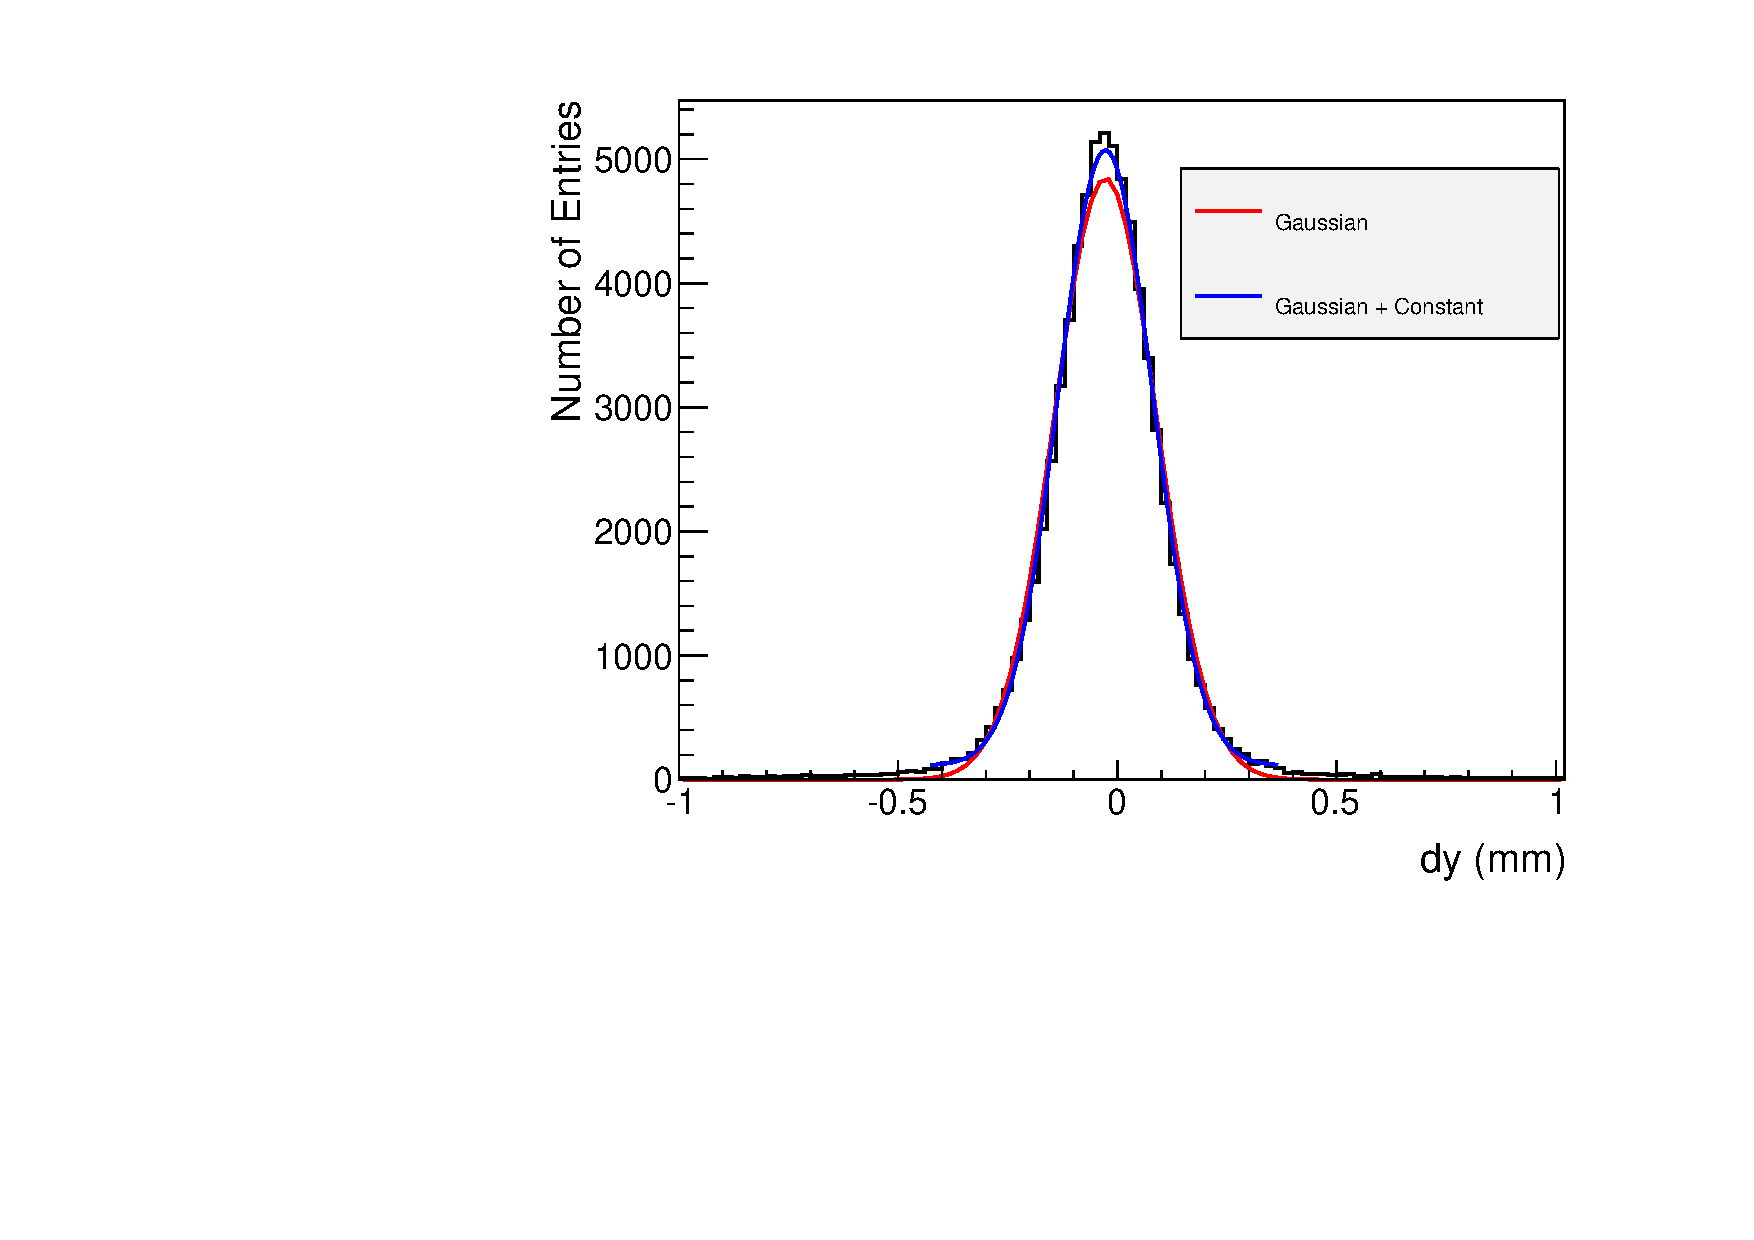
\includegraphics[keepaspectratio=true, width=\textwidth]{Figures/spatialRes_DownY.pdf}
	\caption{Spatial residual of DownY.}
                \label{dx-Y}
        \end{subfigure}
         \caption{Spatial residual distribution of data taken at 4 degrees of tilt around Y coordinate.}
        \label{dx}
\end{figure}

Figure \ref{res} shows the dependence of spatial resolution on the tilt angle. It is seen that the spatial resolution reaches to $\sim 0.15$\myunit{mm} at zero degrees of the incidence angle. The spatial resolution increases with increasing tilt angle (i.e. incidence angle). The particles passes through the detector with an incidence angle leaves broader signal on the readout system, this leads to a wider residual distribution therefore a larger spatial resolution. As expected, the resolution of the layers DownY and UpY increases with larger tilt around X coordinate whereas the resolution of the DownX and UpX do not change (see Figure \ref{res-X}). The same behavior also observed with the data taken by tilting around the Y coordinate (see Figure \ref{res-Y}). 


\begin{figure}[h!]
        \centering
         \begin{subfigure}[t]{0.45\textwidth}
   	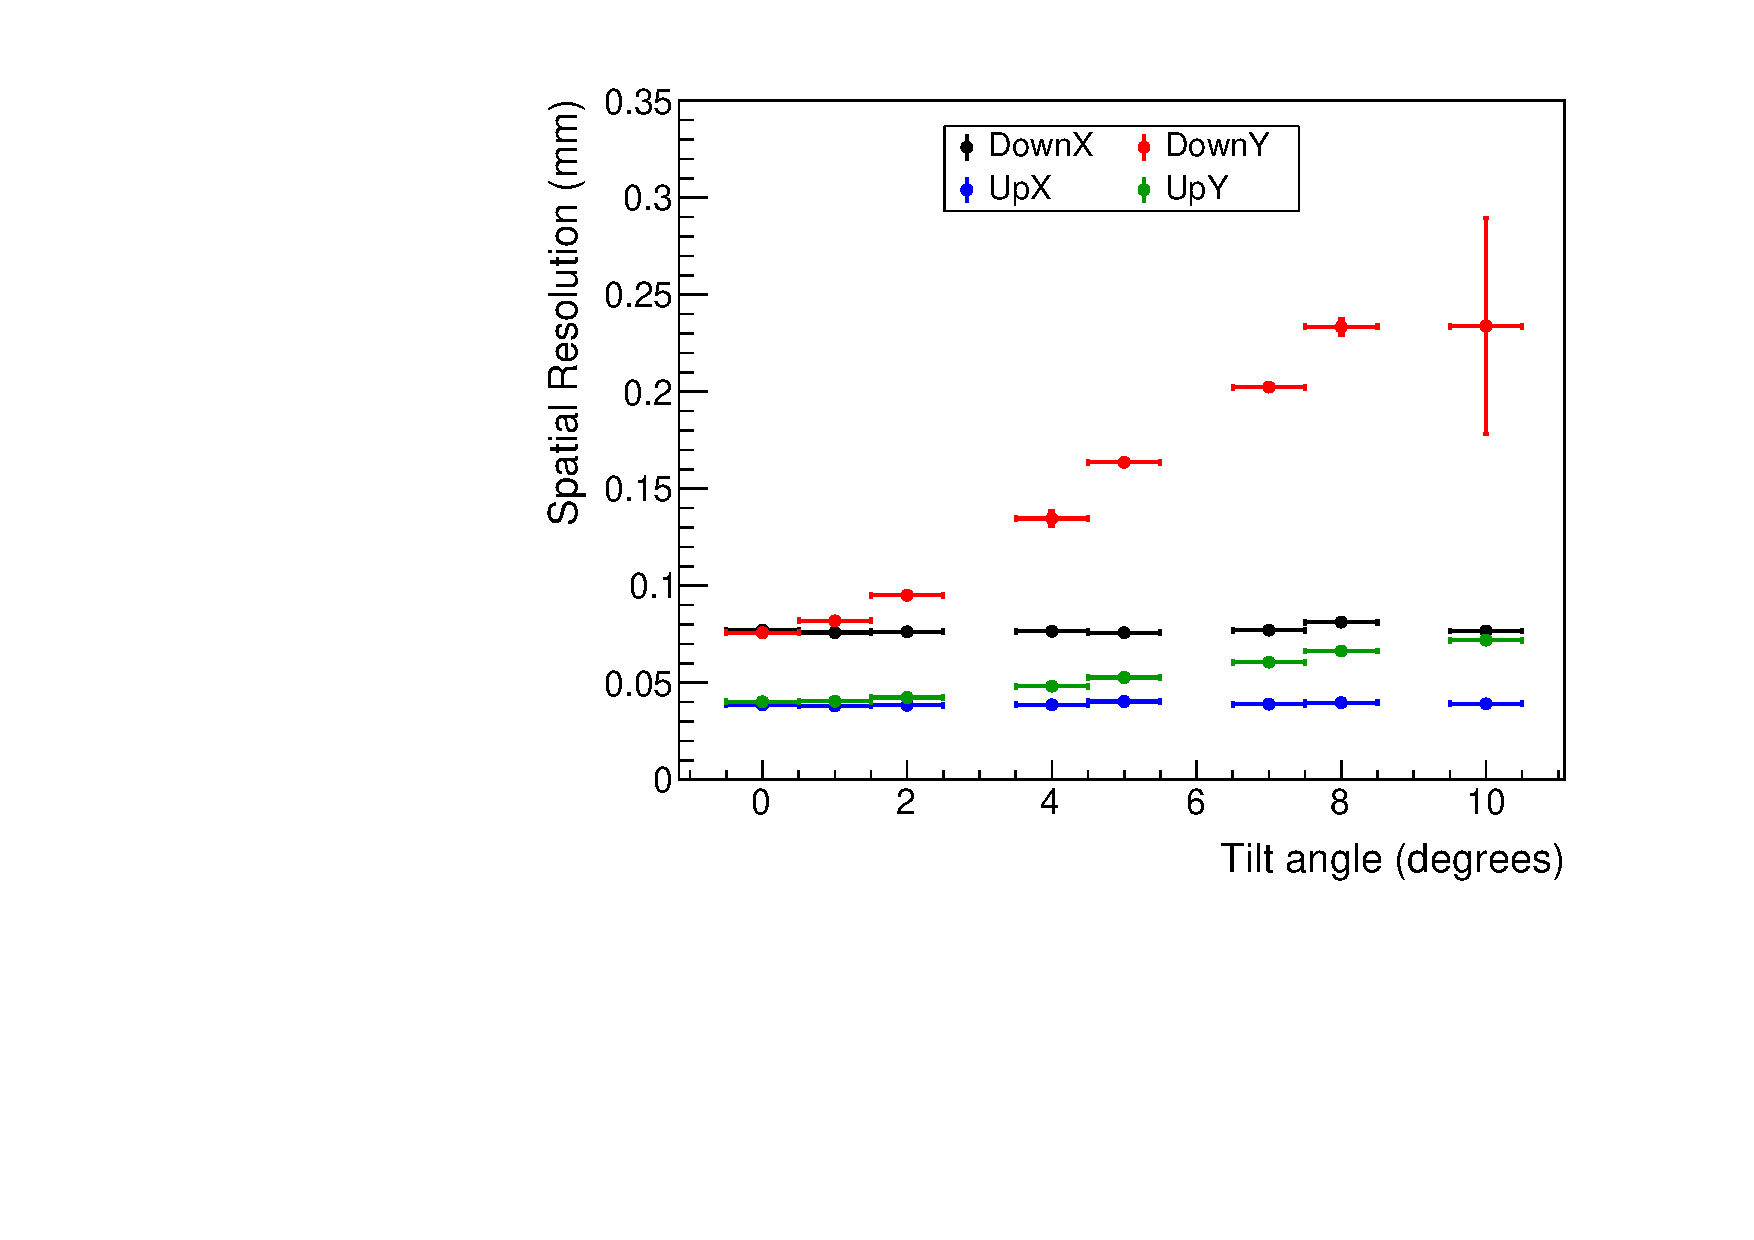
\includegraphics[keepaspectratio=true, width=\textwidth]{Figures/mgr_res_tiltX.pdf}
	\caption{Tilt around X coordinate.}
	\label{res-X}
        \end{subfigure}
         ~
         \begin{subfigure}[t]{0.45\textwidth}
        \centering
   	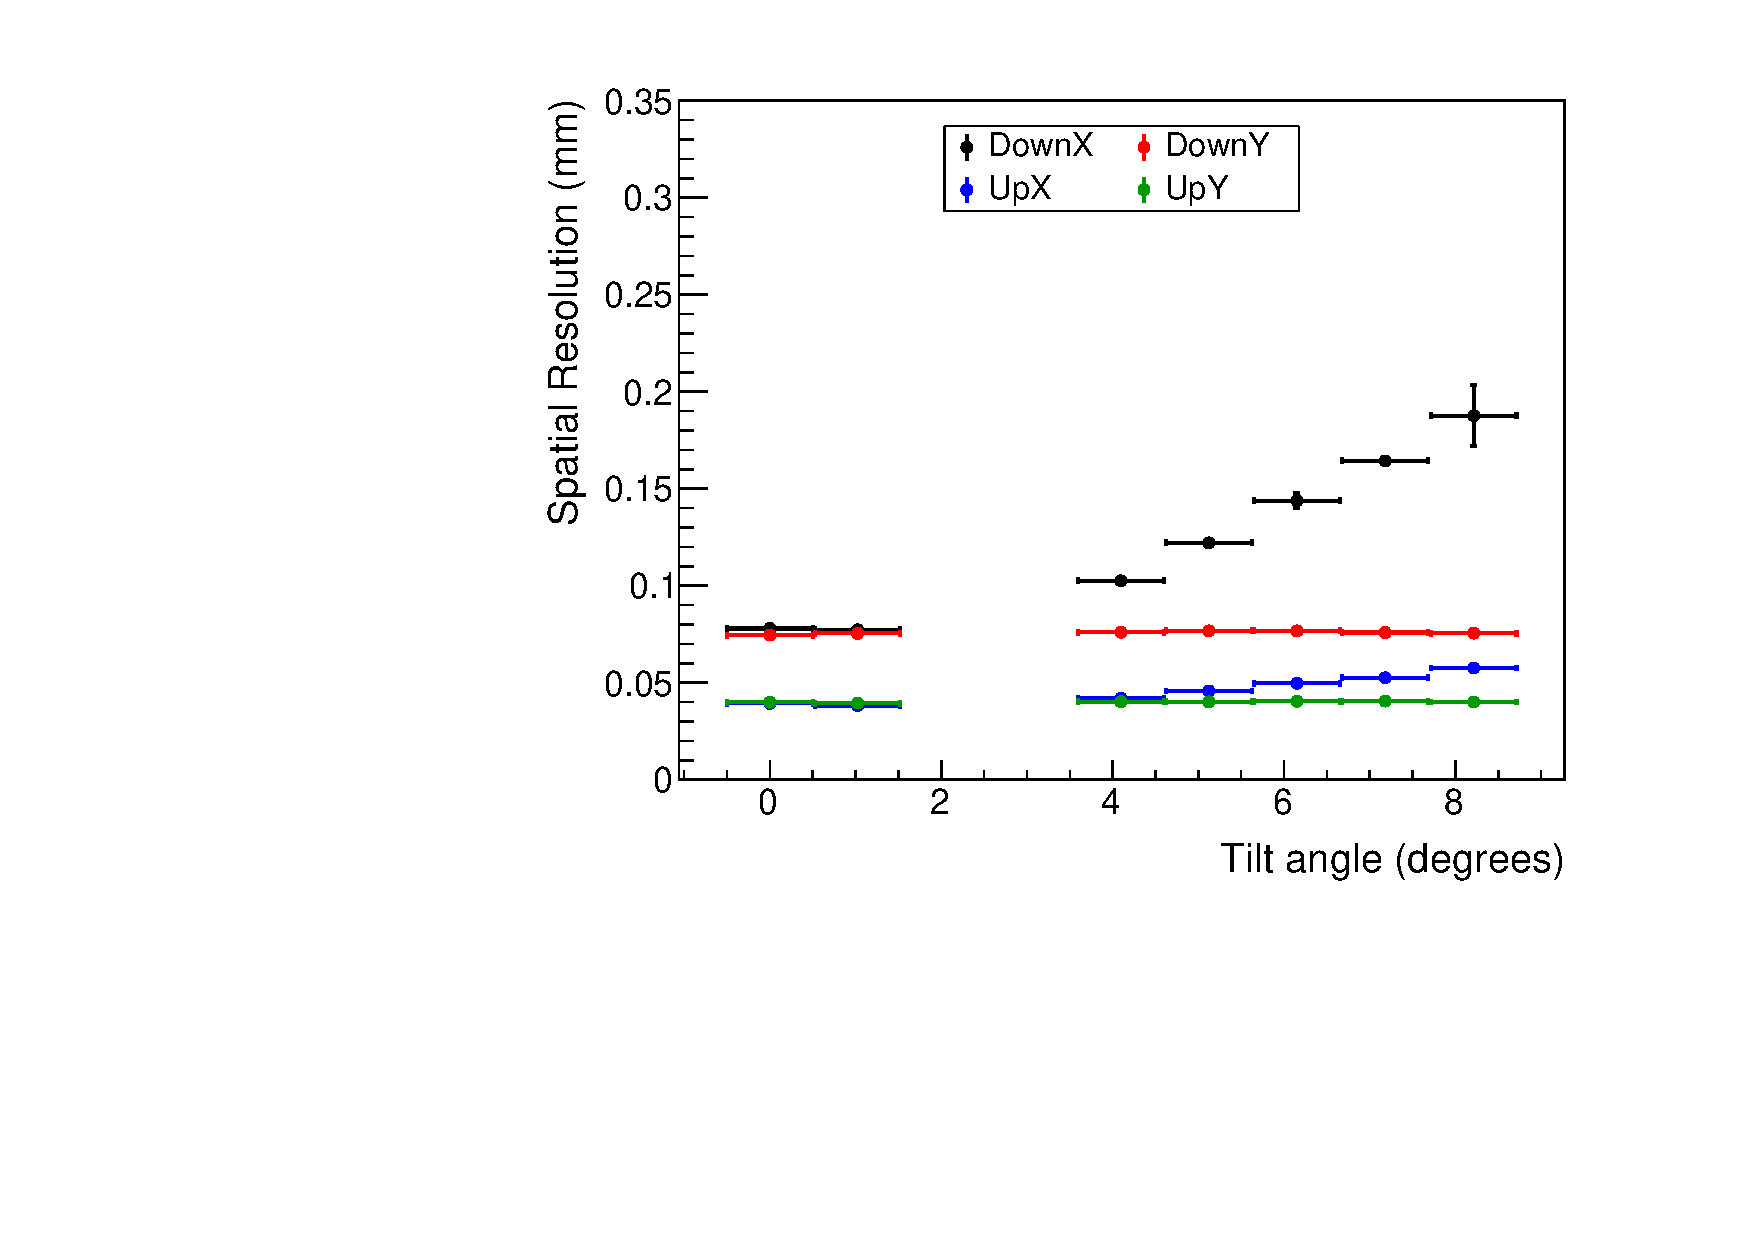
\includegraphics[keepaspectratio=true, width=\textwidth]{Figures/mgr_res_tiltY.pdf}
	\caption{Tilt around Y coordinate.}
                \label{res-Y}
        \end{subfigure}
         \caption{Spatial resolution dependence on tilt angle.}
        \label{res}
\end{figure}


\subsection{Angular Resolution}
The angular resolution is calculated by using the angular residual distribution (Figure \ref{ang-residual}), where d$\theta$ denotes the difference of expected and measured angle of the particle track. The expected angle is calculated by using the 2D hit points of the Reference and the Up layers, where as the angle measured by the Doublet is determined by using the Up and Down layers 2D hits. The Figure \ref{ang-residual}, shows the angular residual distribution of the data taken at 4 degrees of tilt around Y coordinate. The non-zero mean of the distribution is due to the mis-alignment of the layers, however the mis-alignment do not affect the resolution measurement. The same procedure, explained in Section \ref{sec-spa-res}, is applied to calculate the systematic error on the angular resolution measurement. The Figure \ref{ang-resolution} shows the dependence of angular resolution on the tilt angles around X (in black) and Y (in red) coordinates. At zero tilt angle the angular resolution is $\sim 0.5$\myunit{degrees} and increases with increasing tilt angle. 


\begin{figure}[h!]
        \centering
         \begin{subfigure}[t]{0.45\textwidth}
   	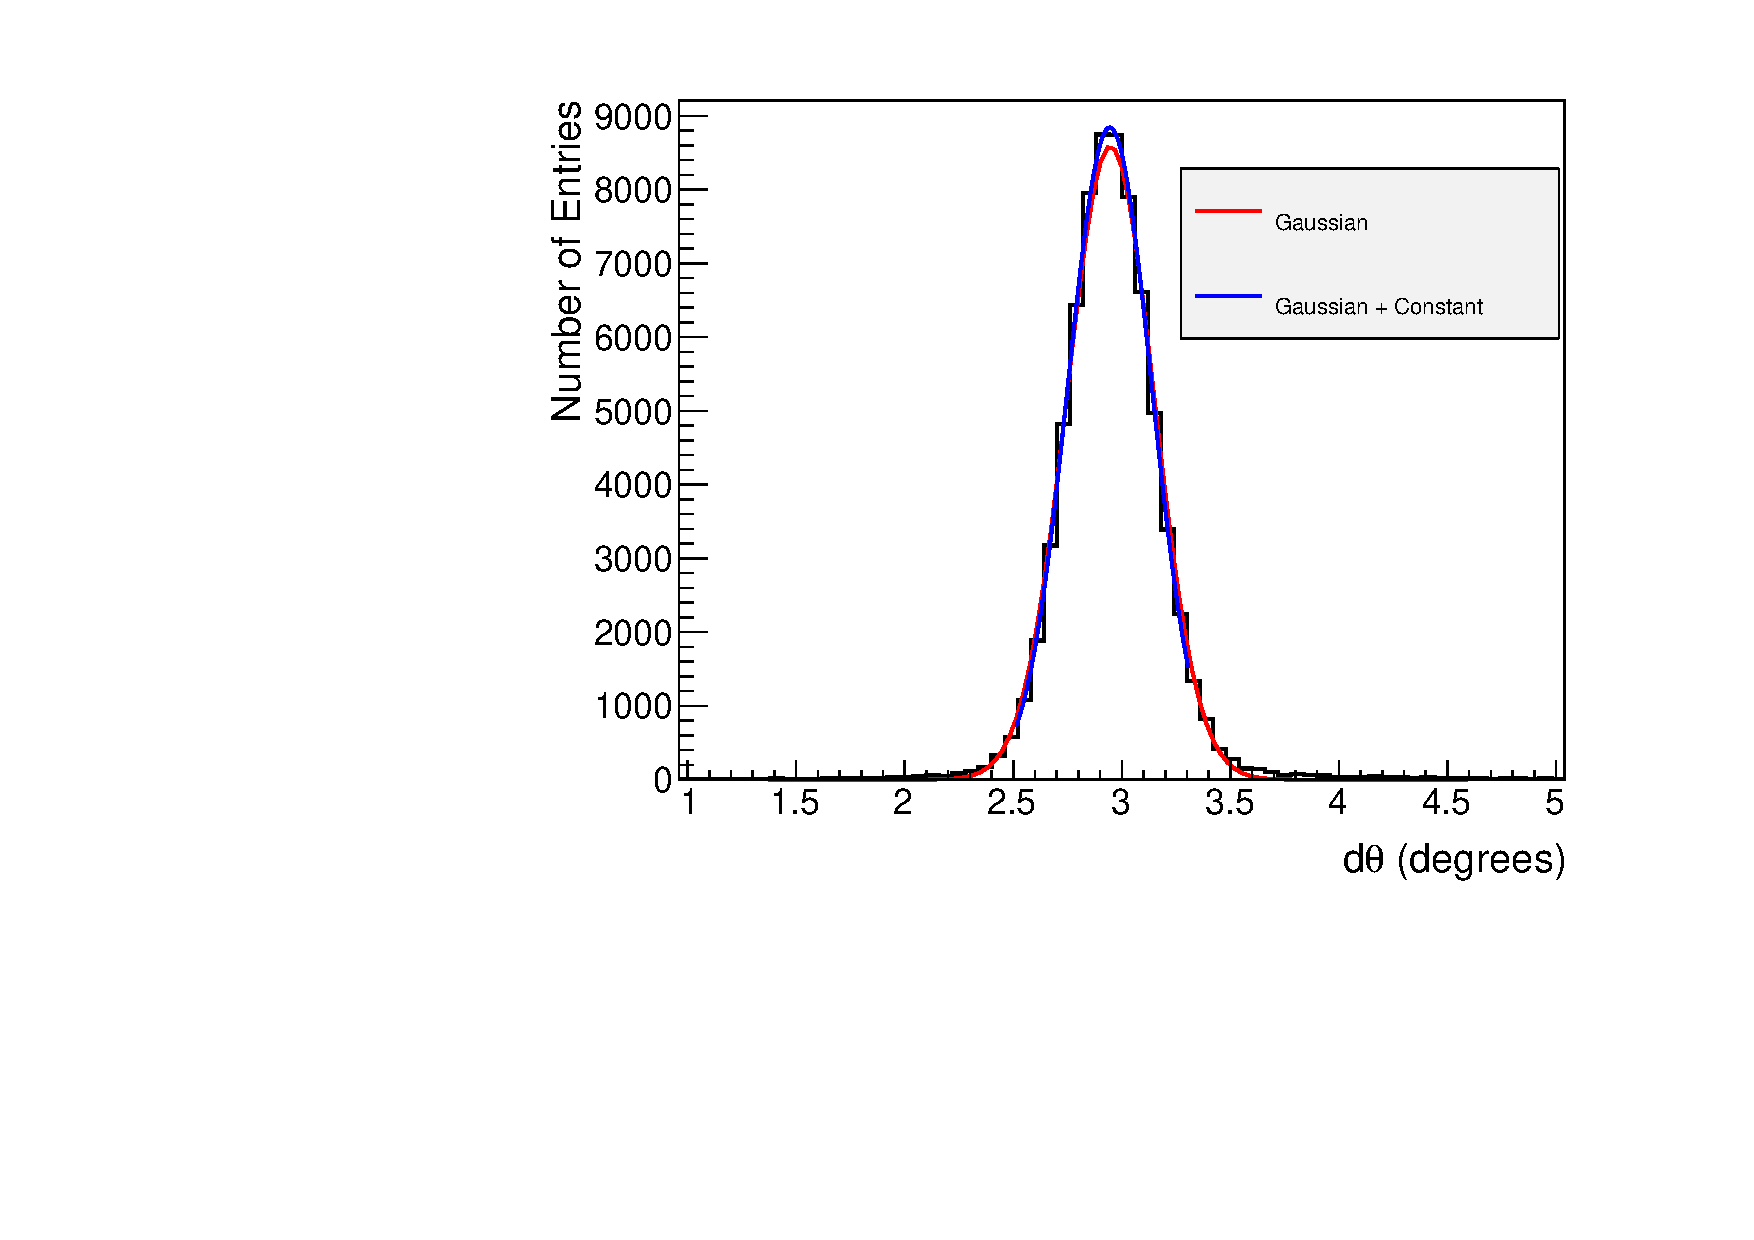
\includegraphics[keepaspectratio=true, width=\textwidth]{Figures/angularRes_Down.pdf}
	\caption{Angular residual distribution of data taken at 4 degrees of tilt around Y coordinate.}
	\label{ang-residual}
        \end{subfigure}
         ~
         \begin{subfigure}[t]{0.45\textwidth}
        \centering
   	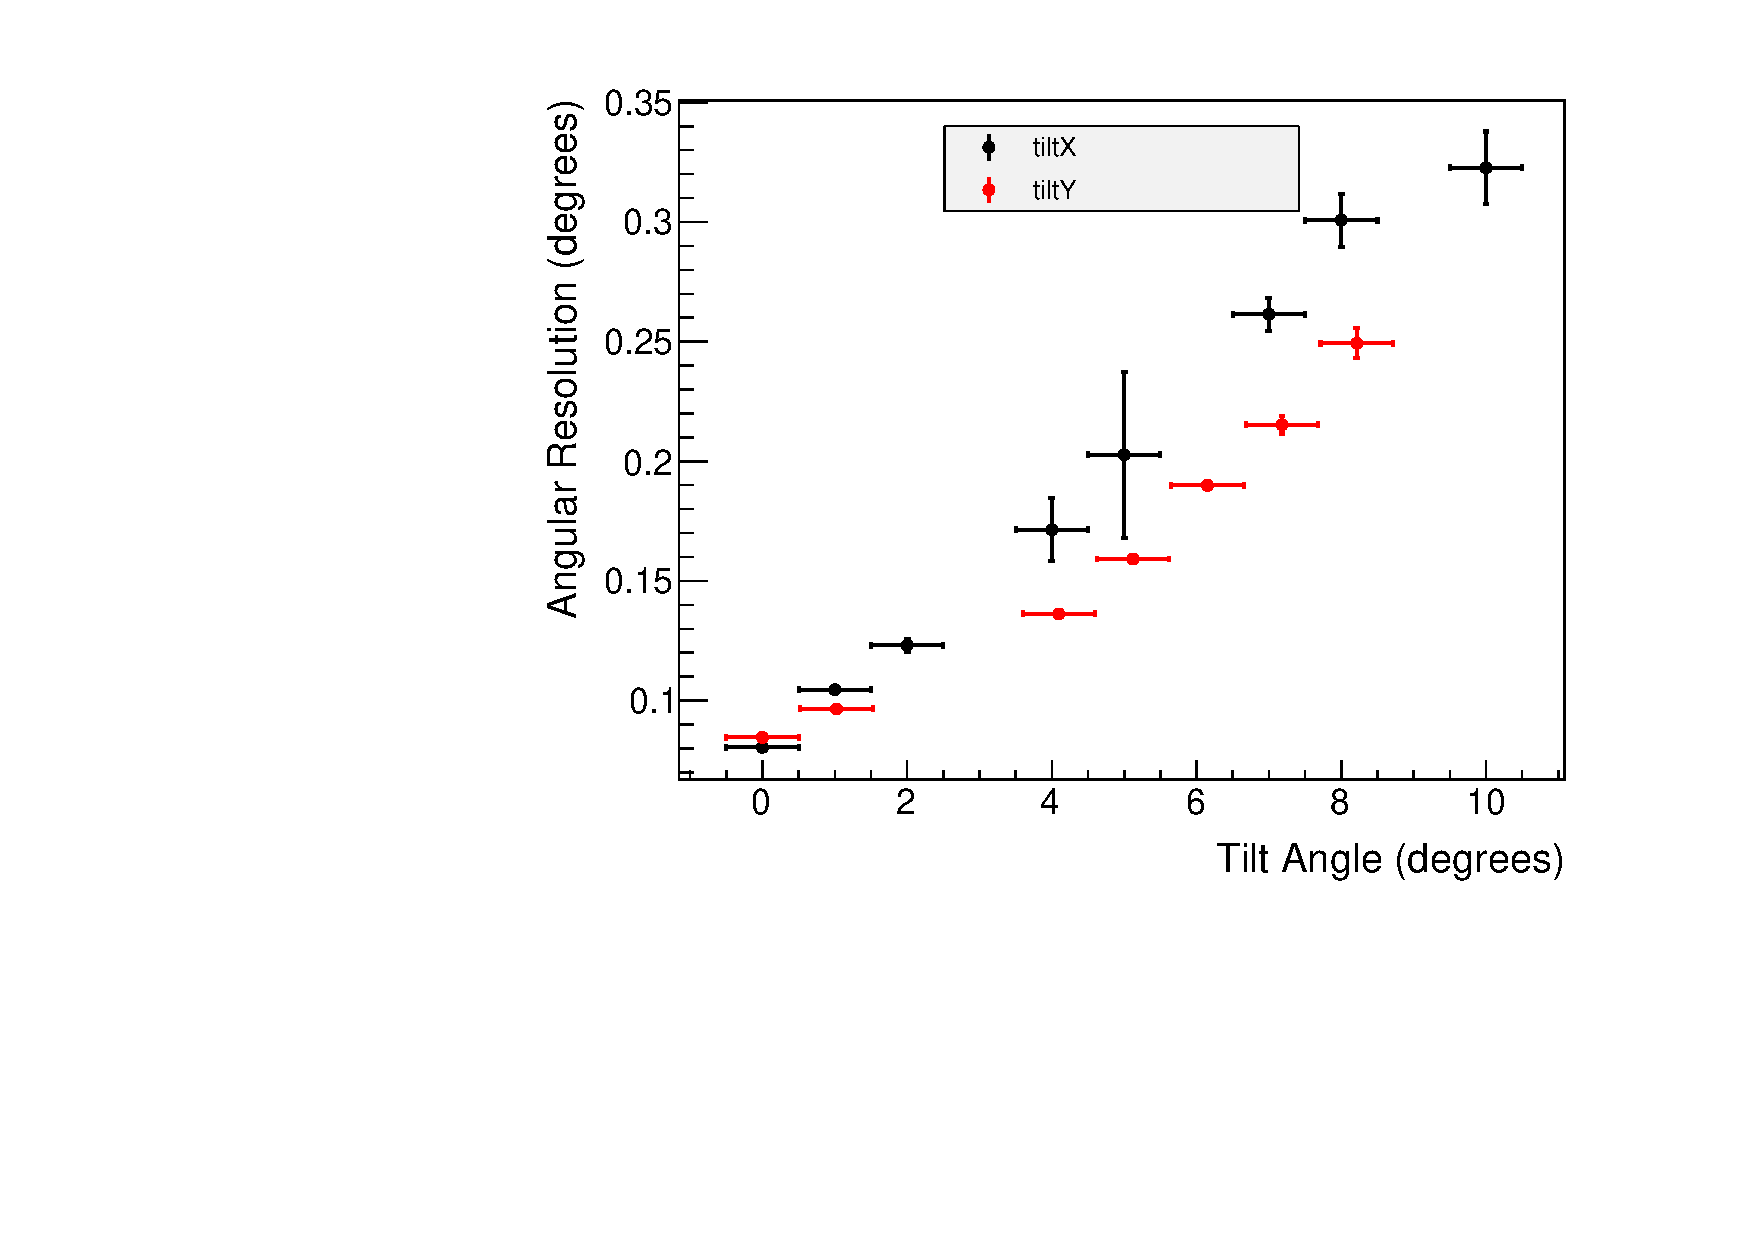
\includegraphics[keepaspectratio=true, width=\textwidth]{Figures/mgr_angres.pdf}
	\caption{Angular resolution dependence on tilt angle.}
                \label{ang-resolution}
        \end{subfigure}
         \caption{Angular resolution.}
        \label{res}
\end{figure}



\section{Conclusion and Outlook}
\label{Sec:Conc}

In this paper, a new type of micromegas detector with two 2D detection layers in a common gas volume is presented and its performance is studied using 4.4\myunit{GeV} electron beam. It is shown that the detector has an efficiency higher than $90\%$ regardless of the incidence beam angle. Its spatial resolution is measured to be around 0.05\myunit{mm} and the angular resolution is $\sim 0.05$\myunit{^\circ} at zero incidence angle. Their dependence on incidence angle of a particle are shown in this paper. 

The performance measurements show that a micromegas detector with two 2D detection layers in a common gas volume is an excellent tracking detector candidate for experiments requires precise spatial and angular resolution; however, has limited space and/or requires low material budget. 


\section*{Acknowledgements}

We would like to acknowledge the close collaboration with XXX. This work is supported by the Volkswagen Foundation and the German Research Foundation (DFG). The measurements leading to electron beam results have been performed at the Test Beam Facility at DESY Hamburg (Germany), a member of the Helmholtz Association (HGF)

\bibliography{MMTwoRegions}

\end{document}
\endinput






















